% Autor: Leonhard Segger, Alexander Neuwirth
% Datum: 2017-10-30
\documentclass[
	% Papierformat
	a4paper,
	% Schriftgröße (beliebige Größen mit „fontsize=Xpt“)
	12pt,
	% Schreibt die Papiergröße korrekt ins Ausgabedokument
	pagesize,
	% Sprache für z.B. Babel
	ngerman
]{scrartcl}

% Achtung: Die Reihenfolge der Pakete kann (leider) wichtig sein!
% Insbesondere sollten (so wie hier) babel, fontenc und inputenc (in dieser
% Reihenfolge) als Erstes und hyperref und cleveref (Reihenfolge auch hier
% beachten) als Letztes geladen werden!

% Silbentrennung etc.; Sprache wird durch Option bei \documentclass festgelegt
\usepackage{babel}
% Verwendung der Zeichentabelle T1 (Sonderzeichen etc.)
\usepackage[T1]{fontenc}
% Legt die Zeichenkodierung der Eingabedatei fest, z.B. UTF-8
\usepackage[utf8]{inputenc}
% Schriftart
\usepackage{lmodern}
% Zusätzliche Sonderzeichen
\usepackage{textcomp}

% Mathepaket (intlimits: Grenzen über/unter Integralzeichen)
\usepackage[intlimits]{amsmath}
% Ermöglicht die Nutzung von \SI{Zahl}{Einheit} u.a.
\usepackage{siunitx}
% Zum flexiblen Einbinden von Grafiken (\includegraphics)
\usepackage{graphicx}
% Abbildungen im Fließtext
\usepackage{wrapfig}
% Abbildungen nebeneinander (subfigure, subtable)
\usepackage{subcaption}
% Funktionen für Anführungszeichen
\usepackage{csquotes}
% Zitieren, Bibliographie
\usepackage{biblatex}

% Verlinkt Textstellen im PDF-Dokument
\usepackage[unicode]{hyperref}
% "Schlaue" Referenzen (nach hyperref laden!)
\usepackage{cleveref}
% Zur Darstellung von Webadressen
\usepackage{url}

% siunitx: Deutsche Ausgabe, Messfehler getrennt mit ± ausgeben
\sisetup{
	locale=DE,
	separate-uncertainty
}

\begin{document}
	\begin{titlepage}
		\centering
		{\scshape\LARGE Versuchsbericht zu \par}
		\vspace{1cm}
		{\scshape\huge S2 -- Experimentieren, und dann?\par}
		\vspace{2.5cm}
		{\LARGE Gruppe 6Mi \par}
		\vspace{0.5cm}
		
		{\large Alexander Neuwirth (E-Mail: a\_neuw01@wwu.de) \par}
		{\large Leonhard Segger (E-Mail: l\_segg03@uni-muenster.de) \par}
		\vfill
		
		durchgeführt am 25.10.2017\par
		betreut von\par
		{\large Dr. Anke \textsc{(Beck-)Schmidt}} \par%Ich hoffe, das ist ok stumpf die zu nehmen.
		{\large Christian \textsc{???}} %Ich hoffe, das ist ok stumpf die zu nehmen.
		
		\vfill
		
		{\large \today\par}
	\end{titlepage}
	\tableofcontents
	
	\newpage
	\section{Einführung}
	
	Die Messung des Ortsfaktor im Physikalischen Institut in Münster ergab einen Wert zwischen 10,5 und 11 \si{m/s^2}. Dabei wurde die Zeit gemessen die eine Metallkugel für eine feste Strecke vertikal zum Boden im freien Fall benötigt. Da dieser Wert eine große Abweichung von dem Erwartungswert der Physikalisch-Technische Bundesanstalt hat (9,813 \si{m/s^2}), stellte sich die Frage, ob der Ortsfaktor für Münster angepasst werden muss.\par
	Um entscheiden zu können, ob eine Änderung des Wertes notwendig ist, wurden mehrere Reproduktionsmessungen durchgeführt. Diese Messungen bestehen aus dem Bestimmen der Zeiten die Fadenpendel verschiedener Längen für eine Periode benötigen.  
	
	\newpage
	\section{Kurzfassung}
	
	\newpage
	\section{Methoden}
	Um den Ortsfaktor mit einem Fadenpendel bestimmen zu können, haben wir die Formel für die Schwingdauer eines Fadenpendels verwendet.
		\begin{equation}\label{eq:Ortsfaktor}
			T_0 = 2\pi \sqrt{\frac{l}{g}}
			\Rightarrow{} g = 4\pi{}^2\frac{l}{T_0^2}
		\end{equation}
	Da diese Formel eine Kleinwinkelnäherung (\(\sin{\varphi} \approx \varphi \)) ist, gilt es zu beachten, dass man das Fadenpendel initial nicht zu weit auslenkt. 
	Des Weiteren haben wir uns entschieden immer die Zeit für 20 Schwingungsperioden zu messen, da sich so der Reaktionsfehler zum Start und Ende der Messung reduzieren lässt.
	Als Anfangs- und Endpunkt unserer Messung haben wir den Ort genommen, in dem sich das Pendel, wenn es nicht schwingt, befindet. Wir haben uns für diesen Punkt entschieden, da sich das Pendel in diesem Punkt genähert mit konstanter Geschwindigkeit bewegt und somit ist es leichter Reaktionsfehler auszugleichen. Ein alternativer Punkt wäre der Wendepunkt des Pendels gewesen, jedoch ist der exakte Zeitpunkt schwerer zu erkennen, da sich das Pendel langsamer bewegt und somit ist der Zeitraum in dem das Pendel erkennbar stillsteht größer.\par
	Sollten zusätzliche Schwingungen in andere Richtungen als die der initialen Auslenkung auftreten, so betrachten wir diese nicht weiter, da wir davon ausgehen, dass diese Schwingungen sich lediglich überlagern und (sofern sie nicht zu groß sind) keine Auswirkung auf die Messung haben.  
	\newpage
	\section{Ergebnisse}
	\subsection{Messungen}
	\subsubsection{Konstante Länge}
	Gemessen wurden 5 x 20 Schwingungen.
	\begin{itemize}
		\item Unsicherheit von \(l\): 
			\begin{itemize}
				\item $\pm0.5\si{cm}$ Abweichung, WDF Dreieck, Standardabweichung (Typ B): \( u_B(l) = \frac{1\si{cm}}{2\sqrt{6}} = 0.2\si{cm} \)
			\end{itemize}

		\item Unsicherheit von \(\bar{T}\): 
			\begin{itemize}
				\item Standardabweichung Mittelwert (Typ A): \( u_A(\bar{T}) = 0.0007\si{s} \)
				\item Reaktionszeit  $\pm0.19 \si{s}$, (Typ B): \( u_B(\bar{T}) = \frac{2\cdot0.19\si{s}}{2\sqrt{3}} = 0.0055\si{s} \)
				\item Komb. Unsicherheit: $ u_C(\bar{T}) = \sqrt{(0.0007\si{s})^2+(0.0055\si{s})^2} = 0.0055 \si{s} $
			\end{itemize}
	\end{itemize}

	\begin{tabular}{l r}
		Länge des Pendels: & \(l = 114 \pm 0.2\si{cm} \) \\
		Mittelwert Schwingungsperiode: & \(\bar{T} = 2.1477 \pm 0.0055\si{s} \) \\
	\end{tabular} 
	

	\par

	\noindent Aus \eqref{eq:Ortsfaktor} folgt $ g = 9.757  \si{m/s^2}$. Die kombinierte Unsicherheit von g ergibt sich aus
	\begin{align*}
		u(g) = g * \sqrt{\left(\frac{u(l)}{l}\right)^2 + \left(2\frac{u(\bar{T})}{\bar{T}}\right)^2} = 0.053 \si{m/s^2} \\
		\Rightarrow{} g = (9.757 \pm 0.053) \si{m/s^2}
	\end{align*}

	Der Ortsfaktor des PTBs 9.813 \si{m/s^2} liegt innerhalb der Abweichung des von uns ermittelten Ortsfaktors. Folglich kann man davon ausgehen, dass bei dem Durchführen des Fallturm-Experiments in Münster ein Fehler unterlaufen ist.

	\newpage
	\subsubsection{Verschiedene Längen}
	Gemessen wurden 2 x 20 Schwingungen.


	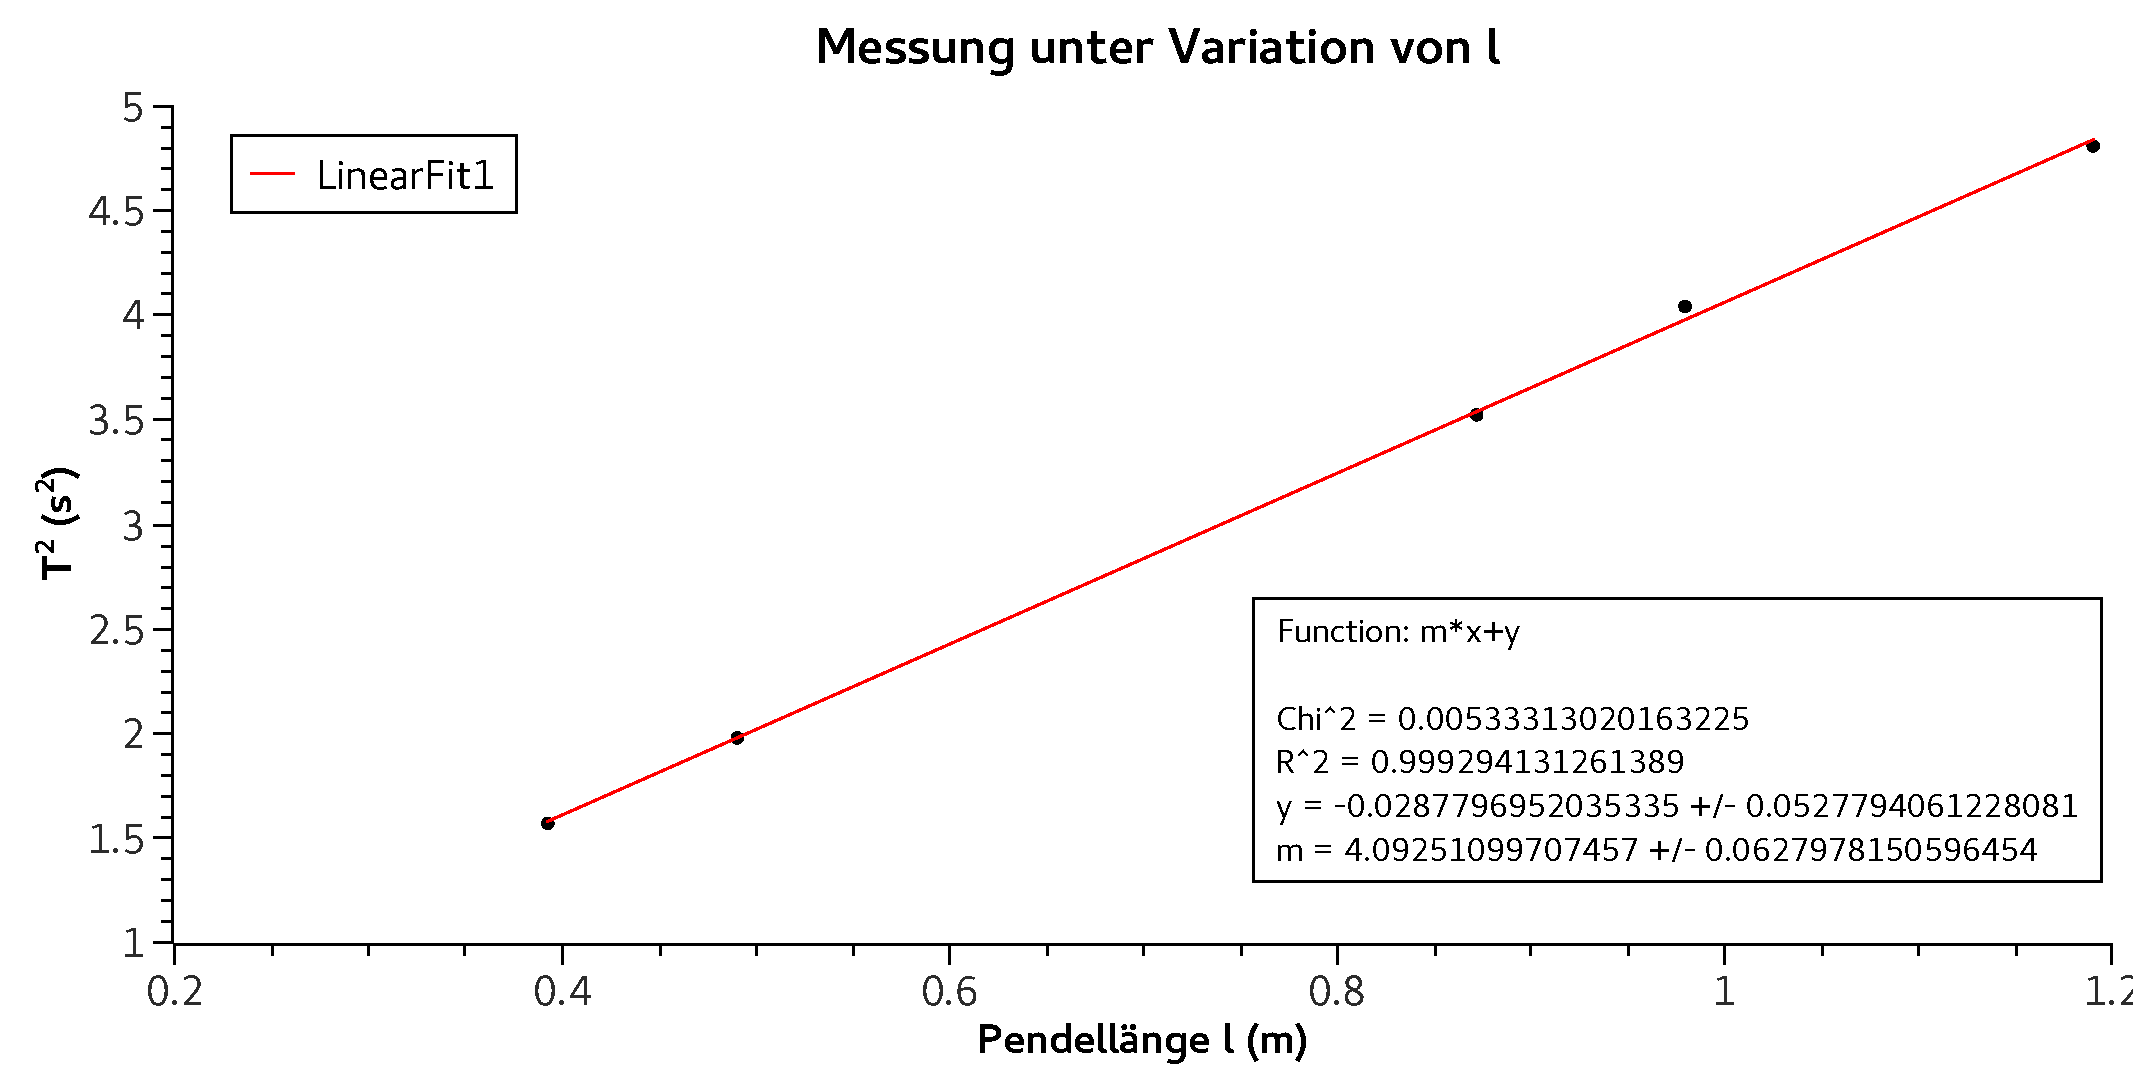
\includegraphics[width=1\textwidth]{Graph}



	\newpage
	\section{Schlussfolgerung}

	
\end{document}
